\chapter{Analisis}
\label{chap:analisis}

Pada bab ini akan dijelaskan mengenai analisis pemanfaatan jsoup untuk mengambil data mahasiswa.

\section{Analisis Pemanfaatan Jsoup}
\label{analisisPemanfaatanJsoup}
Untuk mengambil data mahasiswa, diperlukan sumber data mahasiswa tersebut. Sumber data mahasiswa tersebut dapat diperoleh melalui Portal Akademik Mahasiswa. Portal Akademik Mahasiswa merupakan sebuah situs yang diperuntukkan bagi mahasiswa untuk mendapatkan informasi mengenai profil dan kegiatan akademik mahasiswa tersebut. Mahasiswa dapat mengakses Portal Akademik Mahasiswa melalui \textit{URL} \url{https://studentportal.unpar.ac.id/}. Untuk mengakses Portal Akademik Mahasiswa, mahasiswa harus melakukan \textit{login} menggunakan \textit{email} dan \textit{password} mahasiswa tersebut.

Aplikasi \textit{screensaver} akan melakukan \textit{http request} ke Portal Akademik Mahasiswa untuk mendapatkan data untuk setiap kebutuhan dari masing-masing fitur yang ada, dimana fitur-fitur yang terdapat dalam aplikasi Mahasiswa Wali \textit{Screensaver} adalah informasi umum mengenai mahasiswa, serta prestasi akademik mahasiswa. Pengambilan data secara langsung dari Portal Akademik Mahasiswa dilakukan menggunakan \textit{library} jsoup. Beberapa implementasi pemanfaatan jsoup untuk mengambil data-data tersebut sudah diimplementasikan pada skripsi Andrianto Sugiarto \cite{ifstupor} sebelumnya. Data yang telah didapat dari Portal Akademik Mahasiswa kemudian diolah ke dalam SIAModels, dan ditampilkan sesuai dengan fitur-fitur yang ada pada aplikasi Mahasiswa Wali \textit{Screensaver}.

\subsection{\textit{Login}}
Halaman \textit{Login} (Gambar \ref{fig:3_login} dan \ref{fig:3_login_2}) merupakan halaman dimana mahasiswa memasukkan \textit{email} dan \textit{password} untuk mengakses menu-menu Portal Akademik Mahasiswa.

\begin{figure}[H]
	\centering
	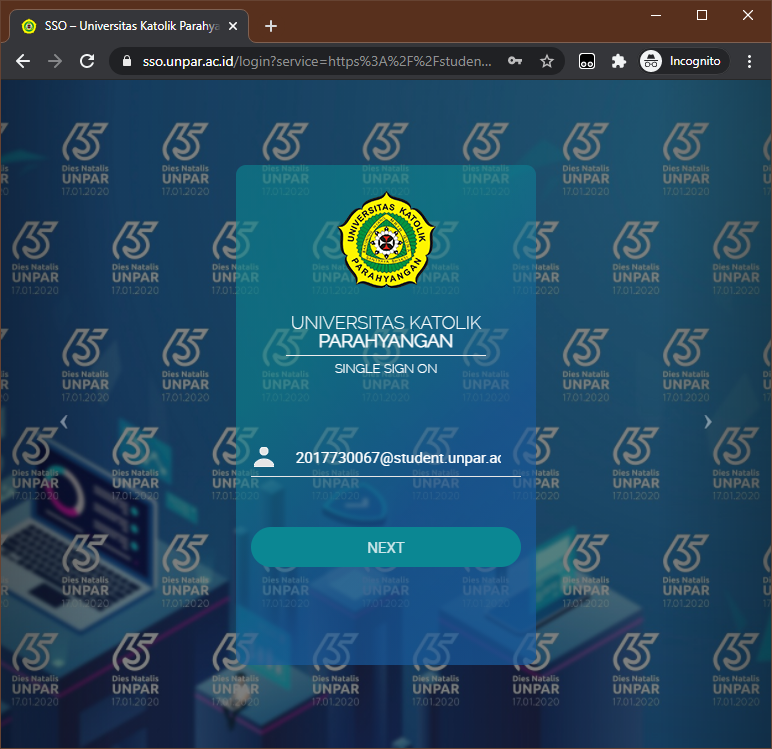
\includegraphics[scale=0.45]{Gambar/login_2.png}
	\caption{Halaman \textit{Login} 1} 
	\label{fig:3_login}
\end{figure}

\begin{figure}[H]
	\centering
	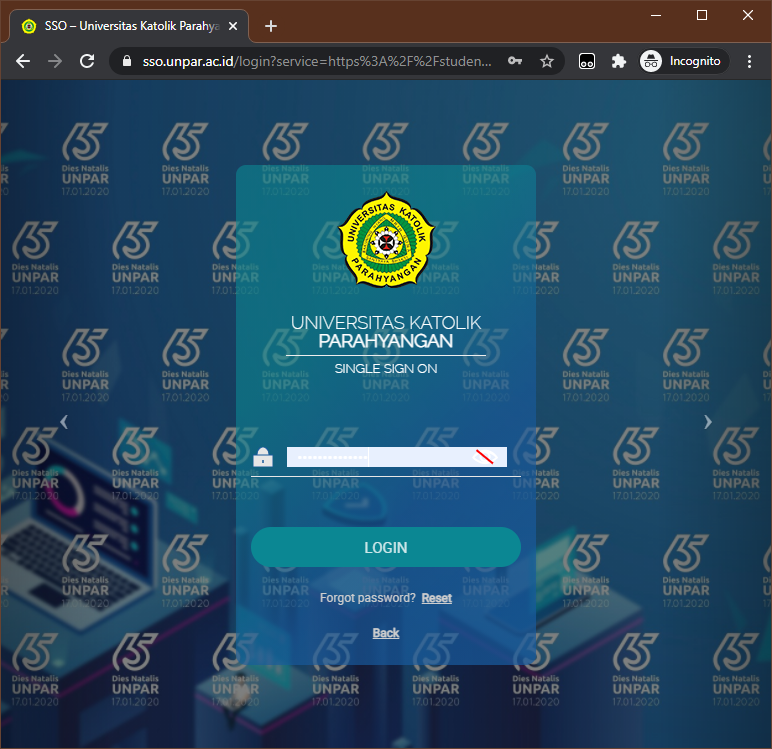
\includegraphics[scale=0.45]{Gambar/login_3.png}
	\caption{Halaman \textit{Login} 2} 
	\label{fig:3_login_2}
\end{figure}

\textit{Login} dilakukan dengan mengirim \textit{request method} POST, dan kemudian mengambil session yang akan digunakan sebagai \textit{cookies} apabila \textit{login} berhasil.
Terdapat beberapa perubahan yang terjadi pada situs Portal Akademik Mahasiswa semenjak skripsi Andrianto Sugiarto \cite{ifstupor}, yang mengakibatkan perlunya perubahan (Kode \ref{diff_login}) terhadap implementasi jsoup:

\begin{enumerate}
    \item Menyimpan atribut mahasiswa pada kelas tersebut agar tidak perlu melakukan \textit{request} \textit{login} berulang kali ketika mengakses menu-menu Portal Akademik Mahasiswa.
    \item Menghapus pemanggilan fungsi validateTLSCertificates() dikarenakan sudah \textit{deprecated} \cite{jsoup}.
    \item Menghapus pengambilan data dengan kueri css "input[name=lt]" dikarenakan kueri tersebut sudah dihapus oleh Portal Akademik Mahasiswa.
    \item Menghapus atribut jsessionid dikarenakan tidak dibutuhkan.
\end{enumerate}

\begin{lstlisting}[language=diff, caption=Perubahan Implementasi Jsoup Login, label=diff_login]
@@ -38,40 +38,32 @@ public class Scraper {
        baseConn.execute();
}

-       public String login(String npm, String pass) throws IOException {
-           init();
-           Mahasiswa logged_mhs = new Mahasiswa(npm);
-           String user = logged_mhs.getEmailAddress();
-           Connection conn = Jsoup.connect(LOGIN_URL);
-           conn.data("Submit", "Login");
-           conn.timeout(0);
-           conn.validateTLSCertificates(false);
-           conn.method(Connection.Method.POST);
-           Response resp = conn.execute();
-           Document doc = resp.parse();
-           String lt = doc.select("input[name=lt]").val();
-           String execution = doc.select("input[name=execution]").val();
-           String jsessionid = resp.cookie("JSESSIONID");
-           /* SSO LOGIN */
-           Connection loginConn = Jsoup.connect(SSO_URL + ";jsessionid=" + jsessionid + "?service=" + LOGIN_URL);
-           loginConn.cookies(resp.cookies());
-           loginConn.data("username", user);
-           loginConn.data("password", pass);
-           loginConn.data("lt", lt);
-           loginConn.data("execution", execution);
-           loginConn.data("_eventId", "submit");
-           loginConn.data("submit", "");
-           loginConn.timeout(0);
-           loginConn.validateTLSCertificates(false);
-           loginConn.method(Connection.Method.POST);
-           resp = loginConn.execute();
-           if (resp.body().contains(user)) {
-                   Map<String, String> phpsessid = resp.cookies();
-                   return phpsessid.get("ci_session");
-           } else {
-                   return null;
-           }
-       }
+       public void login() throws IOException {
+           init();
+           this.mahasiswa = new Mahasiswa(this.npm);
+           String user = this.mahasiswa.getEmailAddress();
+           Connection conn = Jsoup.connect(LOGIN_URL);
+           conn.data("Submit", "Login");
+           conn.timeout(0);
+           conn.method(Connection.Method.POST);
+           Response resp = conn.execute();
+           Document doc = resp.parse();
+           String execution = doc.select("input[name=execution]").val();
+
+           /* SSO LOGIN */
+           Connection loginConn = Jsoup.connect(SSO_URL + "?service=" + LOGIN_URL);
+           loginConn.data("username", user);
+           loginConn.data("password", this.password);
+           loginConn.data("execution", execution);
+           loginConn.data("_eventId", "submit");
+           loginConn.timeout(0);
+           loginConn.method(Connection.Method.POST);
+           resp = loginConn.execute();
+           if (resp.body().contains(user)) {
+               Map<String, String> sessionId = resp.cookies();
+               this.session = sessionId.get("ci_session");
+           }
+       }
\end{lstlisting}

\subsection{Halaman Utama}
Pada Halaman Utama Portal Akademik Mahasiswa (Gambar \ref{fig:3_home}), terdapat nama lengkap dan foto dari mahasiswa tersebut yang dapat diambil dan digunakan. Nama mahasiswa dapat diambil dengan mencari elemen "div" yang memiliki kelas "namaUser d-none d-lg-block mr-3", sehingga kueri css yang dihasilkan adalah "div[class=namaUser d-none d-lg-block mr-3]". Foto mahasiswa dapat diambil dengan mencari elemen "img" yang memiliki kelas "img-fluid fotoProfil", sehingga kueri css yang dihasilkan adalah "img[class=img-fluid fotoProfil]".
Terdapat beberapa perubahan (Kode \ref{diff_halaman_utama}) yang perlu dilakukan terhadap skripsi Andrianto Sugiarto \cite{ifstupor}:

\begin{figure}[H]
	\centering
	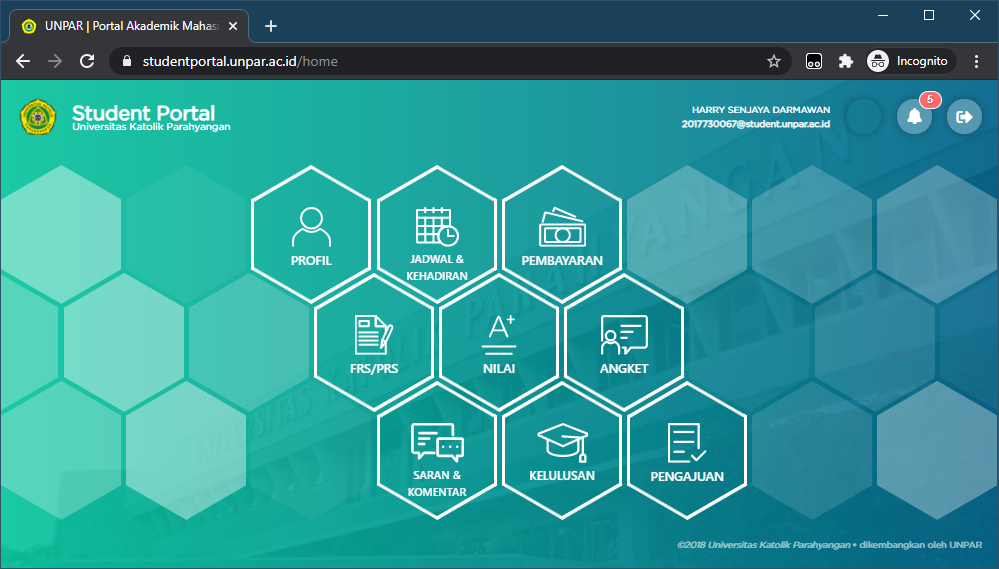
\includegraphics[scale=0.5]{Gambar/home.png}
	\caption{Halaman Utama Portal Akademik Mahasiswa} 
	\label{fig:3_home}
\end{figure}

\begin{enumerate}
    \item Menghapus pemanggilan fungsi validateTLSCertificates() dikarenakan sudah \textit{deprecated} \cite{jsoup}.
    \item Menyimpan atribut mahasiswa pada kelas tersebut agar tidak perlu melakukan \textit{request} \textit{login} berulang kali ketika mengakses menu-menu Portal Akademik Mahasiswa.
    % \item Sebelumnya semester yang sedang dijalani mahasiswa diambil dari menu FRS/PRS, namun karena terdapat perubahan pada Portal Akademik Mahasiswa maka semester yang sedang dijalani mahasiswa diambil dari menu Nilai.
    \item Menghapus pengambilan semester yang sedang dijalani karena tidak akan ditampilkan pada \textit{screensaver}.
\end{enumerate}

\begin{lstlisting}[language=diff, caption=Perubahan Implementasi Jsoup Halaman Utama, label=diff_halaman_utama]
@@ -73,31 +73,20 @@ public class Scraper {
        }
}

-       public TahunSemester requestNamePhotoTahunSemester(String phpsessid, Mahasiswa mhs) throws IOException {
+       public void requestNamePhotoTahunSemester(String phpsessid) throws IOException {
            Connection connection = Jsoup.connect(HOME_URL);
-           connection.cookie("ci_session", phpsessid);
-           connection.timeout(0);
-           connection.validateTLSCertificates(false);
-           connection.method(Connection.Method.GET);
-           Response resp = connection.execute();
-           Document doc = resp.parse();
-           String nama = doc.select("div[class=namaUser d-none d-lg-block mr-3]").text();
-           mhs.setNama(nama.substring(0, nama.indexOf(mhs.getEmailAddress())));
-           Element photo = doc.select("img[class=img-fluid fotoProfil]").first();
-           String photoPath = photo.attr("src");
-           mhs.setPhotoPath(photoPath);
-           connection = Jsoup.connect(NILAI_URL);
-           connection.cookie("ci_session", phpsessid);
-           connection.timeout(0);
-           connection.validateTLSCertificates(false);
-           connection.method(Connection.Method.GET);
-           resp = connection.execute();
-           doc = resp.parse();
-           Elements options = doc.getElementsByAttributeValue("name", "dropdownSemester").first().children();
-           String curr_sem = options.last().val();
-           curr_sem = curr_sem.substring(2,4).concat(curr_sem.substring(5));
-           TahunSemester currTahunSemester = new TahunSemester(curr_sem);
-           return currTahunSemester;
+           connection.cookie("ci_session", phpsessid);
+           connection.timeout(0);
+           connection.method(Connection.Method.GET);
+           Response resp = connection.execute();
+
+           Document doc = resp.parse();
+           String nama = doc.select("div[class=namaUser d-none d-lg-block mr-3]").text();
+           this.mahasiswa.setNama(nama.substring(0, nama.indexOf(this.mahasiswa.getEmailAddress())));
+
+           Element photo = doc.select("img[class=img-fluid fotoProfil]").first();
+           String photoPath = photo.attr("src");
+           this.mahasiswa.setPhotoPath(photoPath);
        }
\end{lstlisting}

Pada halaman utama Portal Akademik Mahasiswa juga terdapat beberapa menu yang dapat digunakan sebagai sumber data yaitu:

\subsection{Profil}
    Menu Profil merupakan halaman yang menampilkan data diri mahasiswa (Gambar \ref{fig:3_profil}). Pada halaman ini tanggal lahir mahasiswa akan diambil untuk ditampilkan pada \textit{screensaver}. Implementasi jsoup tersebut belum diimplementasikan pada skripsi Andrianto Sugiarto \cite{ifstupor}, sehingga perlu dilakukan penambahan fitur untuk mengambil data tersebut. Tanggal lahir mahasiswa dapat diambil dengan mencari elemen "div" yang memiliki kelas "offset-md-1 col-md-10 col-12 headerWrapper my-0 border-bottom", sehingga kueri css yang dihasilkan adalah "div[class=offset-md-1 col-md-10 col-12 headerWrapper my-0 border-bottom]".
    \begin{figure}[H]
    	\centering
    	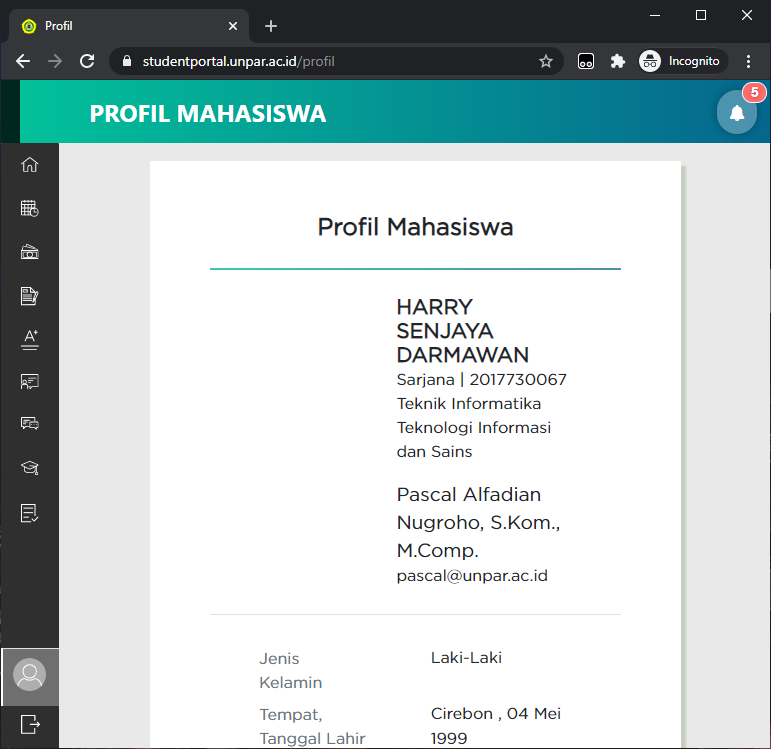
\includegraphics[scale=0.45]{Gambar/profil.png}
    	\caption{Halaman Profil} 
    	\label{fig:3_profil}
    \end{figure}

\subsection{Jadwal}
    Menu Jadwal terdiri dari beberapa submenu:
		\begin{itemize}
		    \item Kehadiran\\
		    Submenu ini berfungsi untuk menandakan kehadiran mahasiswa di suatu mata kuliah pada hari dimana mahasiswa tersebut mengakses halaman tersebut (Gambar \ref{fig:3_kehadiran}).
		    \begin{figure}[H]
    			\centering
    			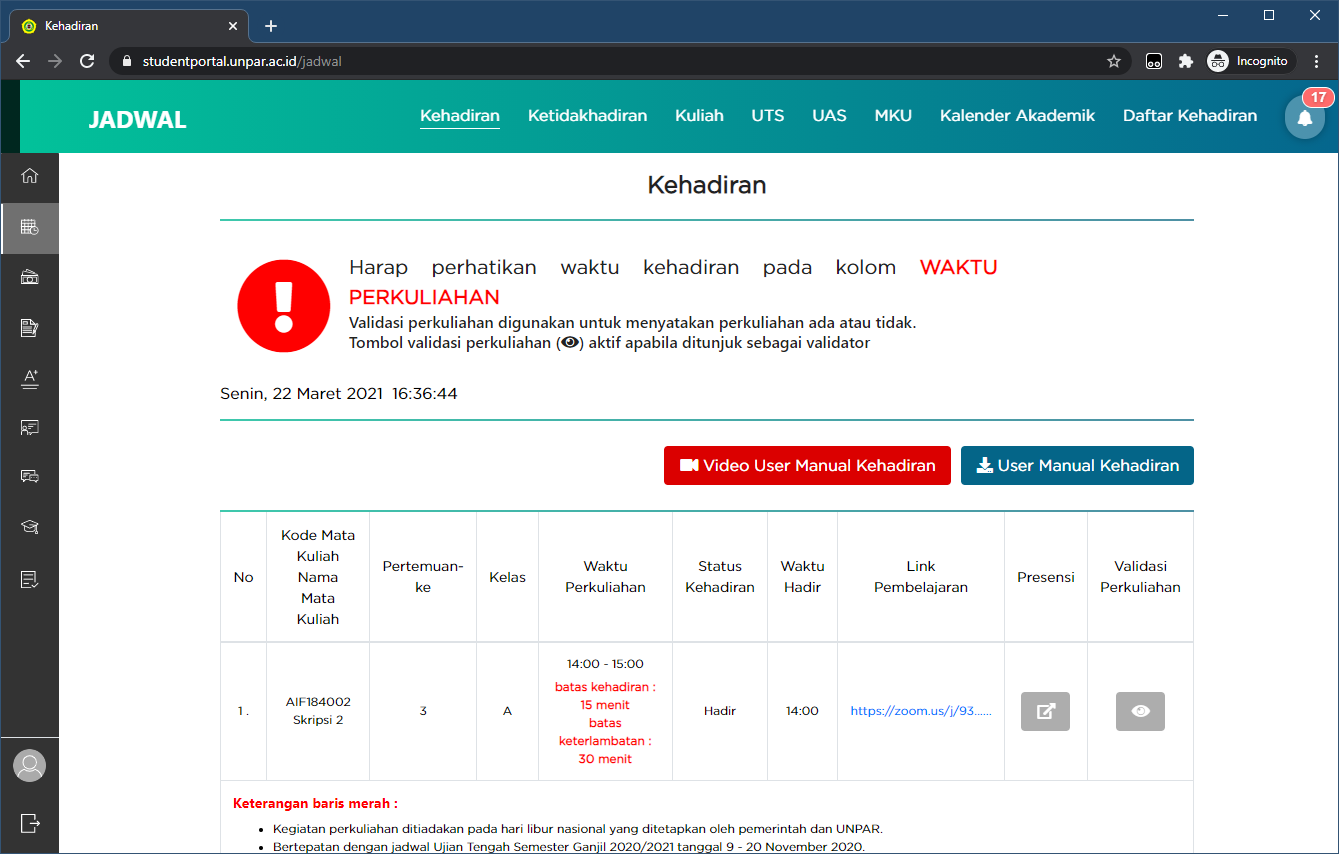
\includegraphics[scale=0.45]{Gambar/jadwal_kehadiran.png}
    			\caption{Halaman Kehadiran}
    			\label{fig:3_kehadiran}
			\end{figure}
			\item Ketidakhadiran\\
		    Submenu ini berfungsi untuk mengunggah surat sakit atau surat izin mahasiswa. (Gambar \ref{fig:3_ketidakhadiran}).
		    \begin{figure}[H]
    			\centering
    			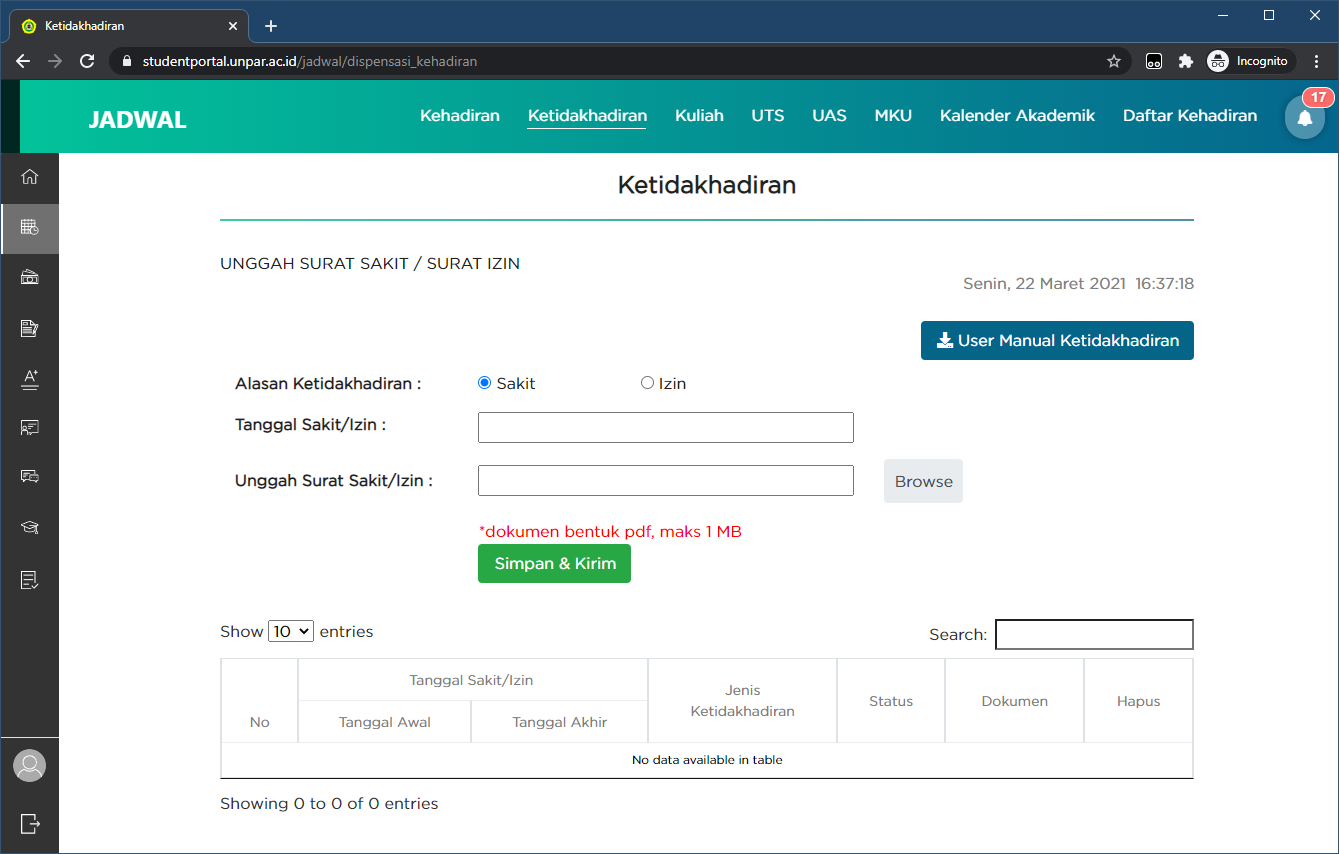
\includegraphics[scale=0.45]{Gambar/jadwal_ketidakhadiran.png}
    			\caption{Halaman Ketidakhadiran}
    			\label{fig:3_ketidakhadiran}
			\end{figure}
			\item Kuliah \\
			Submenu ini berisi tentang jadwal kuliah yang dapat disusun per semester dan terdapat 2 tampilan, yaitu tabel waktu (Gambar \ref{fig:3_jadwal_kuliah}) dan tabel biasa (Gambar \ref{fig:3_jadwal_kuliah_table}).
			\begin{figure}[H]
    			\centering
    			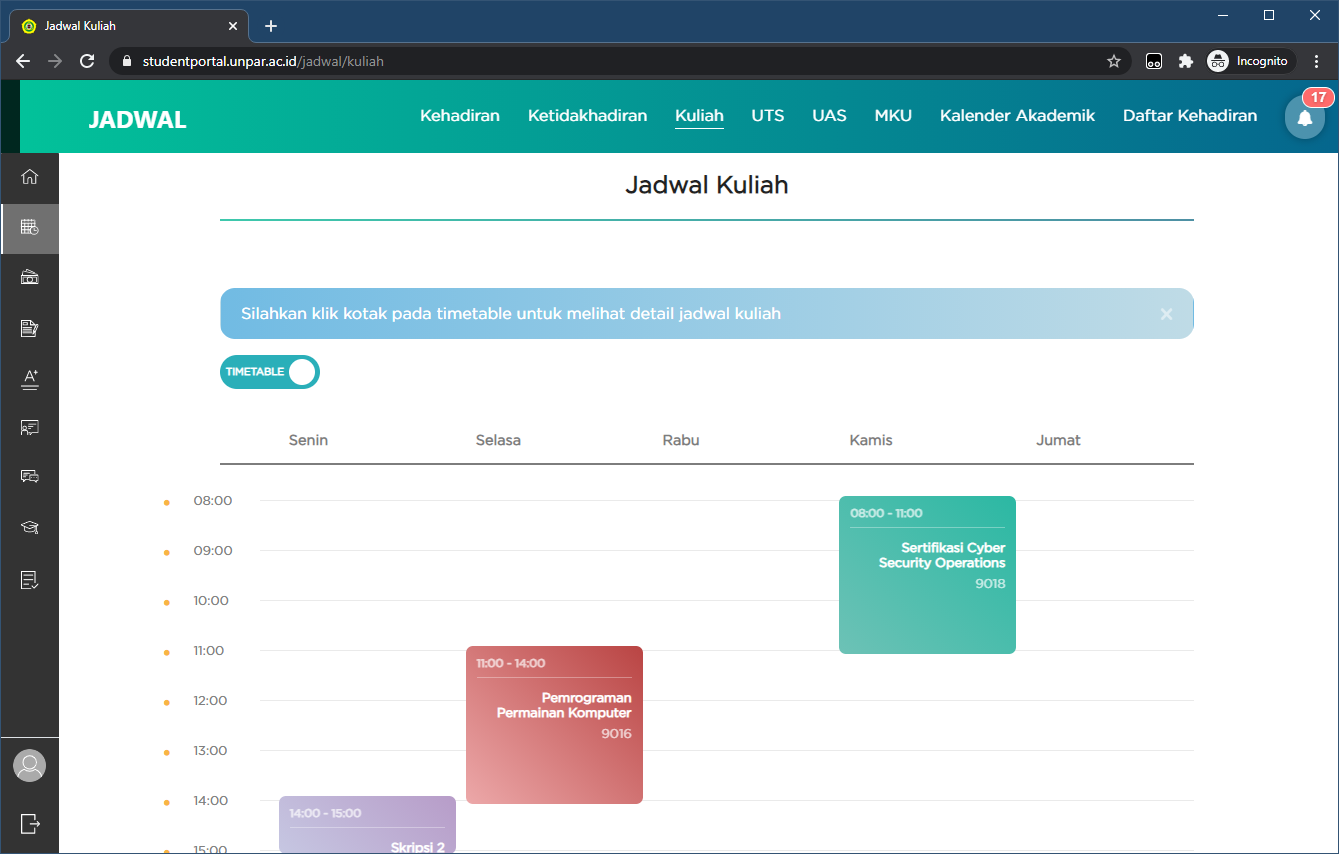
\includegraphics[scale=0.45]{Gambar/jadwal_kuliah.png}
    			\caption{Halaman Jadwal Kuliah Dalam Tabel Waktu}
    			\label{fig:3_jadwal_kuliah}
			\end{figure}
			\begin{figure}[H]
    			\centering
    			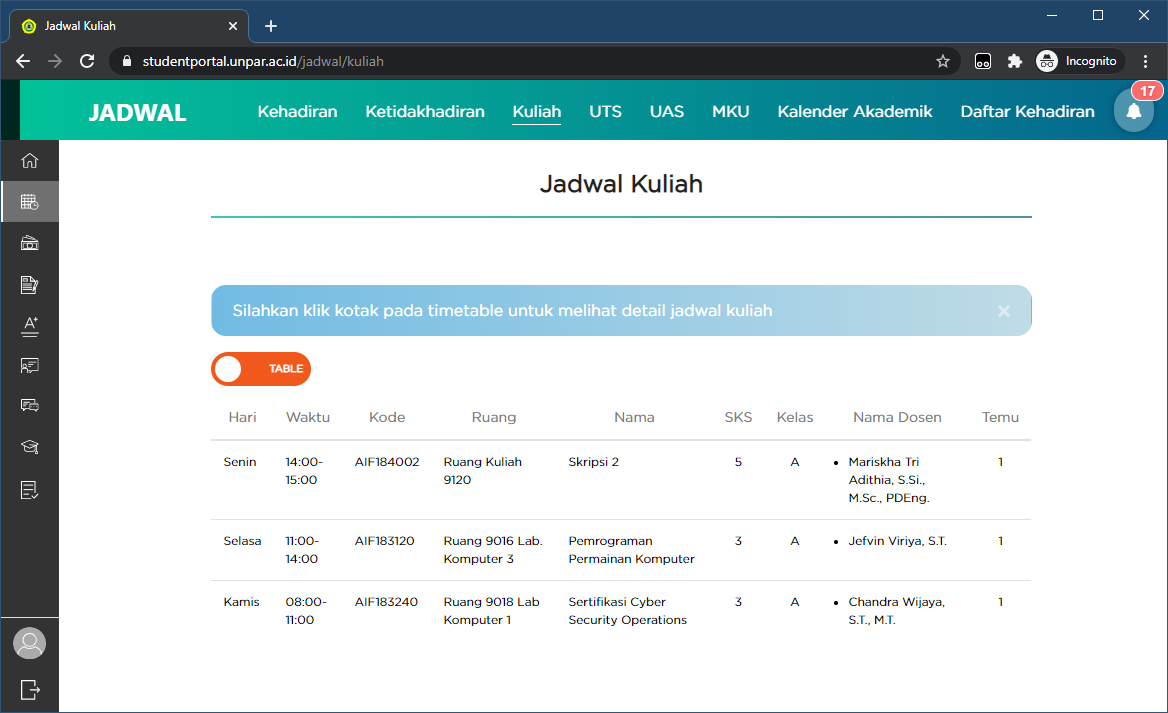
\includegraphics[scale=0.45]{Gambar/jadwal_kuliah_table.png}
    			\caption{Halaman Jadwal Kuliah Tabel}
    			\label{fig:3_jadwal_kuliah_table}
			\end{figure}
			\item UTS \\
			Submenu ini berisi tentang UTS yang dapat disusun per semester (Gambar \ref{fig:3_uts}).
			\begin{figure}[H]
    			\centering
    			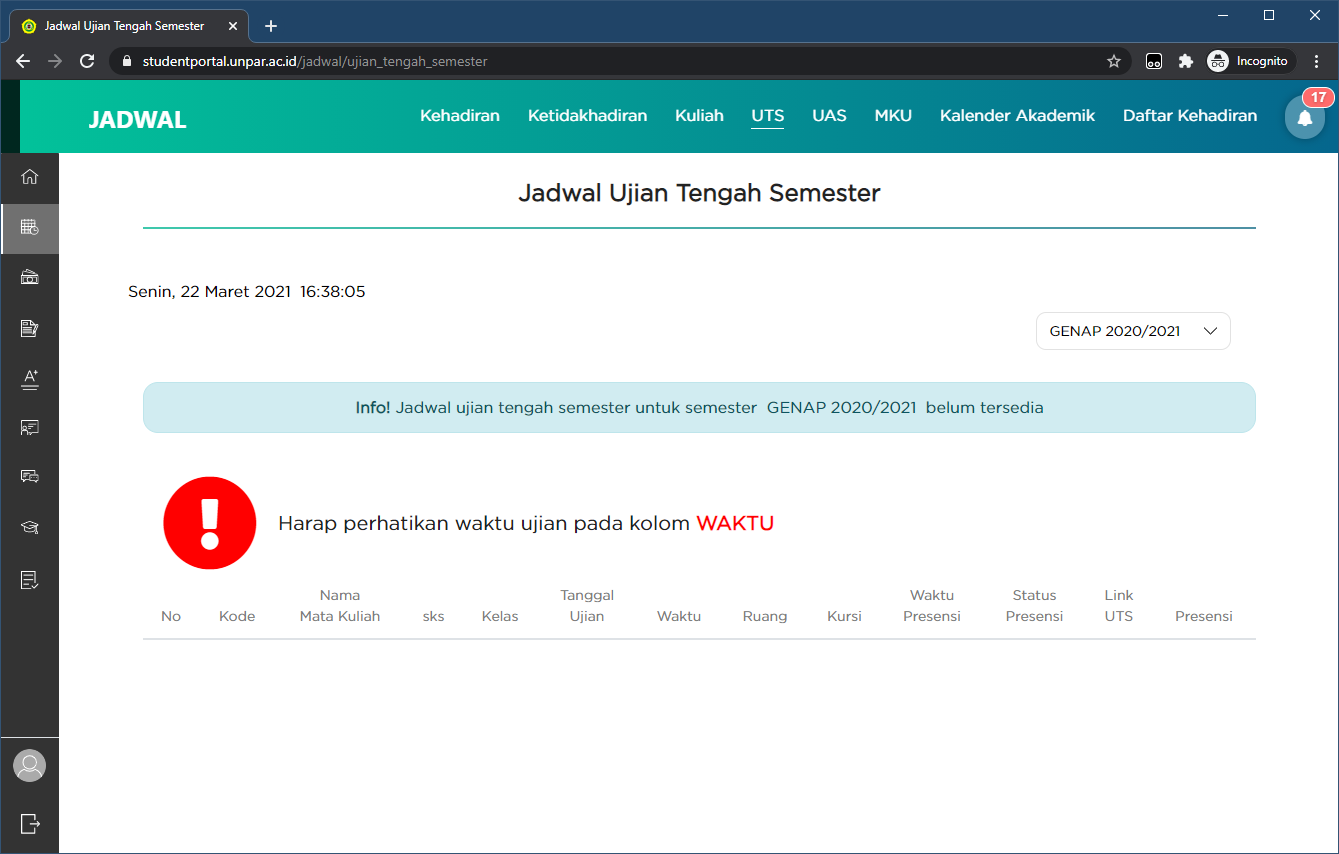
\includegraphics[scale=0.45]{Gambar/jadwal_uts.png}
    			\caption{Halaman UTS}
    			\label{fig:3_uts}
			\end{figure}
			\item UAS \\
			Submenu ini berisi tentang UAS yang dapat disusun per semester (Gambar \ref{fig:3_uas}).
			\begin{figure}[H]
    			\centering
    			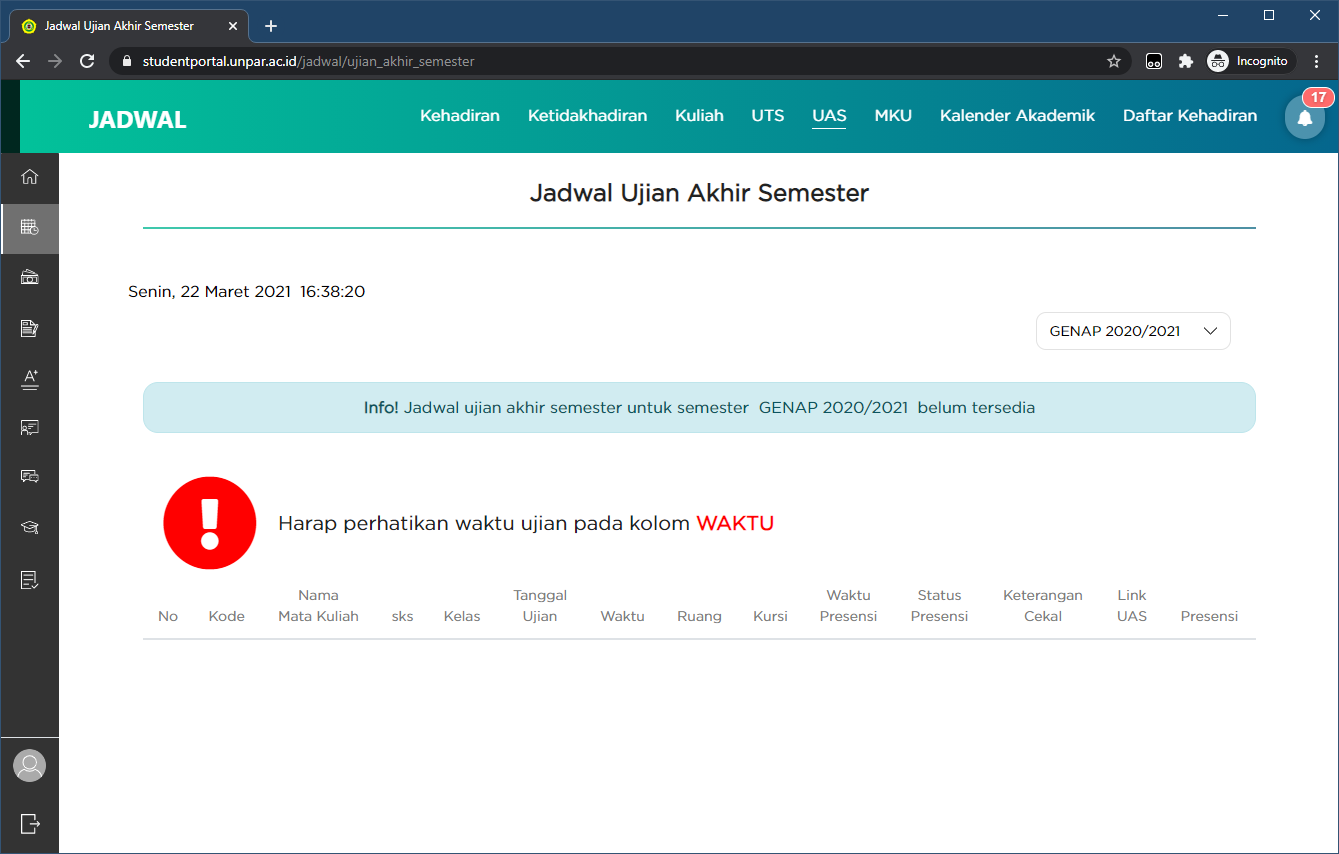
\includegraphics[scale=0.45]{Gambar/jadwal_uas.png}
    			\caption{Halaman UAS}
    			\label{fig:3_uas}
			\end{figure}
			\item MKU \\
			Submenu ini menampilkan seluruh jadwal Mata Kuliah Umum (MKU) yang memberikan informasi tentang kelas-kelas yang dibuka oleh Pusat Kajian Humaniora (PKH) (Gambar \ref{fig:3_mku}).
			\begin{figure}[H]
    			\centering
    			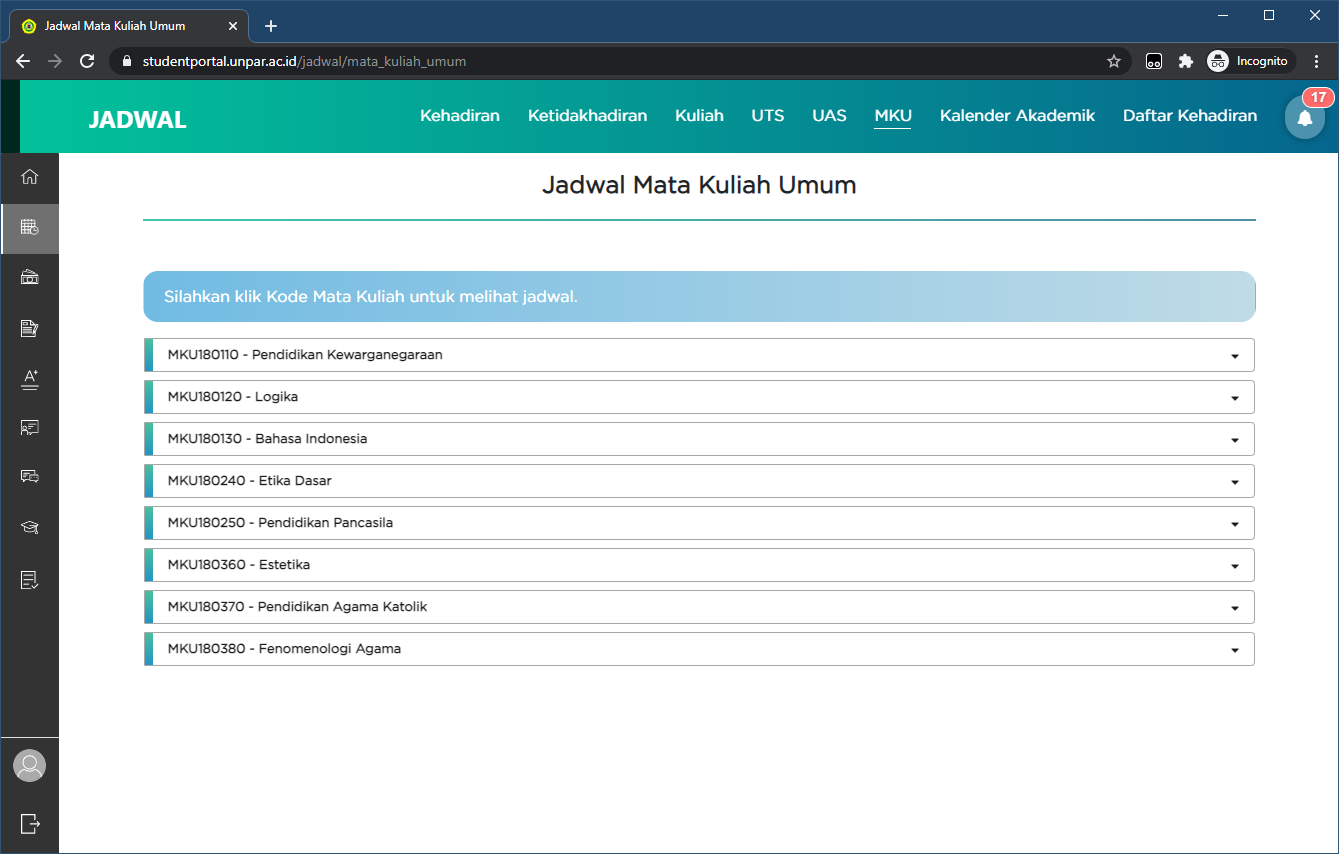
\includegraphics[scale=0.45]{Gambar/jadwal_mku.png}
    			\caption{Halaman MKU}
    			\label{fig:3_mku}
			\end{figure}
			\item Kalender Akademik \\
			Submenu ini menampilkan informasi mengenai kalender akademik UNPAR (Gambar \ref{fig:3_kalender_akademik}).
			\begin{figure}[H]
    			\centering
    			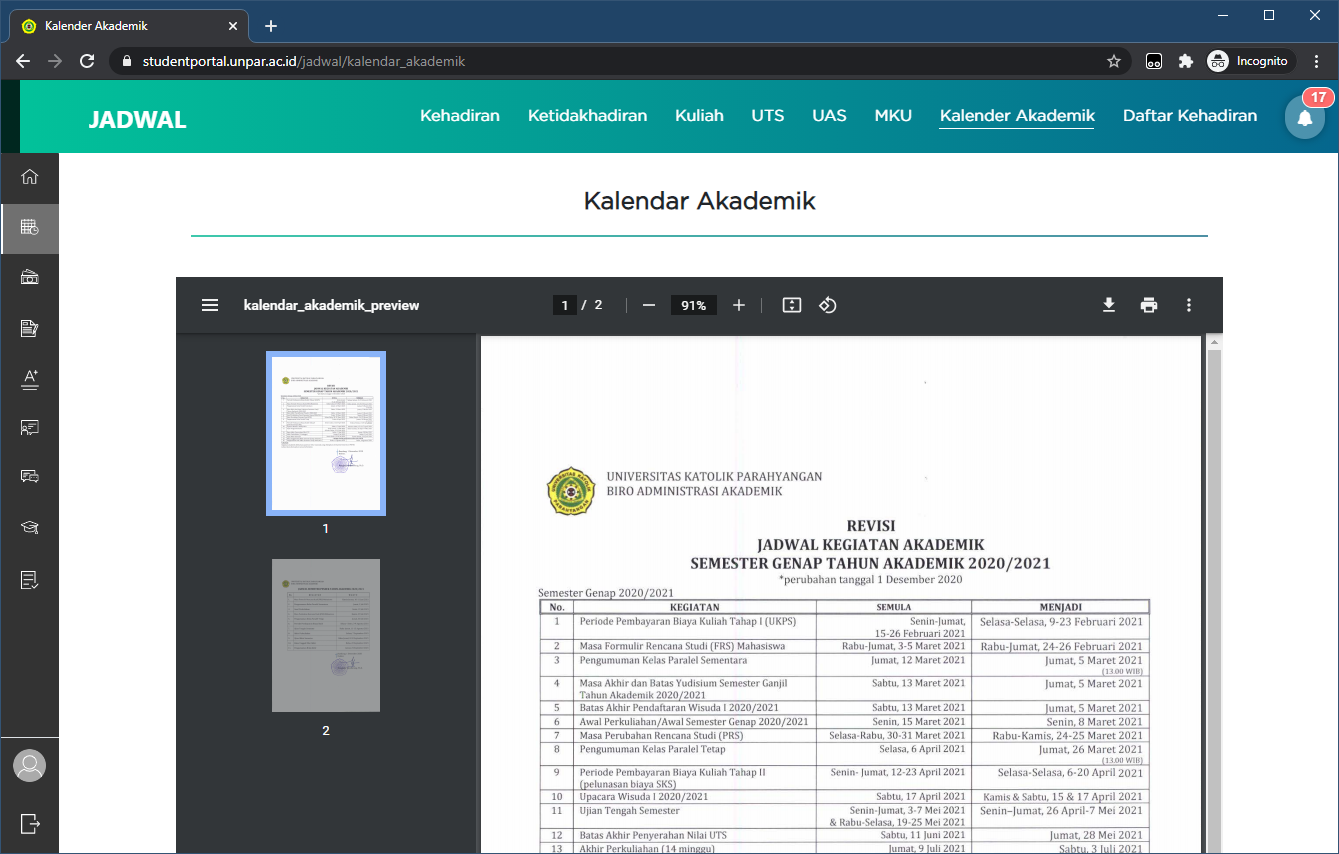
\includegraphics[scale=0.45]{Gambar/jadwal_kalenderakademik.png}
    			\caption{Halaman Kalender Akademik}
    			\label{fig:3_kalender_akademik}
			\end{figure}
			\item Daftar Kehadiran \\
			Submenu ini menampilkan informasi mengenai daftar kehadiran mahasiswa pada setiap mata kuliah yang dapat disusun per semester (Gambar \ref{fig:3_daftar_kehadiran}).
			\begin{figure}[H]
    			\centering
    			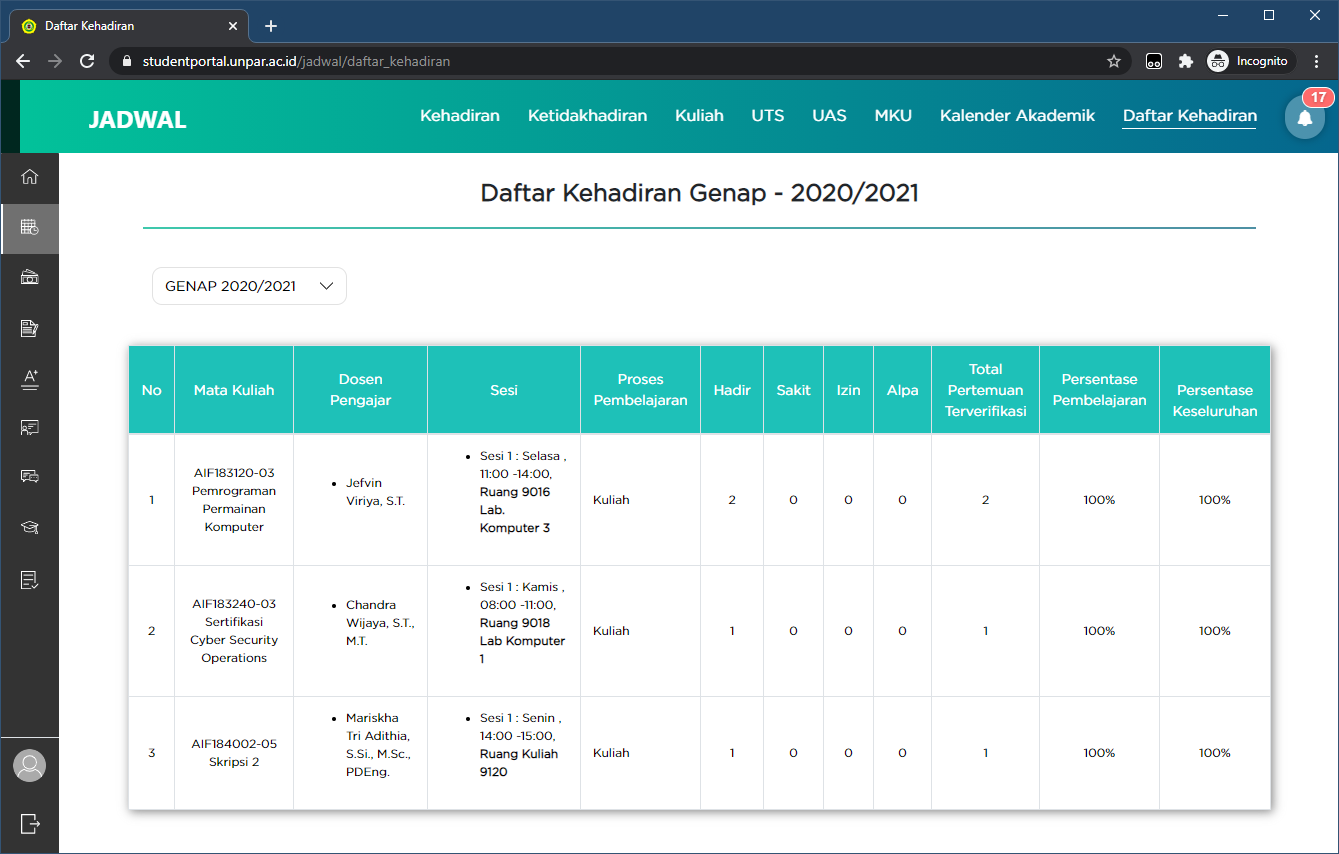
\includegraphics[scale=0.45]{Gambar/jadwal_daftarkehadiran.png}
    			\caption{Halaman Daftar Kehadiran}
    			\label{fig:3_daftar_kehadiran}
			\end{figure}
		\end{itemize}
    
\subsection{Pembayaran}
    Menu ini berfungsi untuk melihat data tagihan pembayaran uang kuliah, riwayat pembayaran, dan keterangan cara-cara pembayaran uang kuliah yang dapat disusun per semester (Gambar \ref{fig:3_pembayaran}).
	\begin{figure}[H]
		\centering
		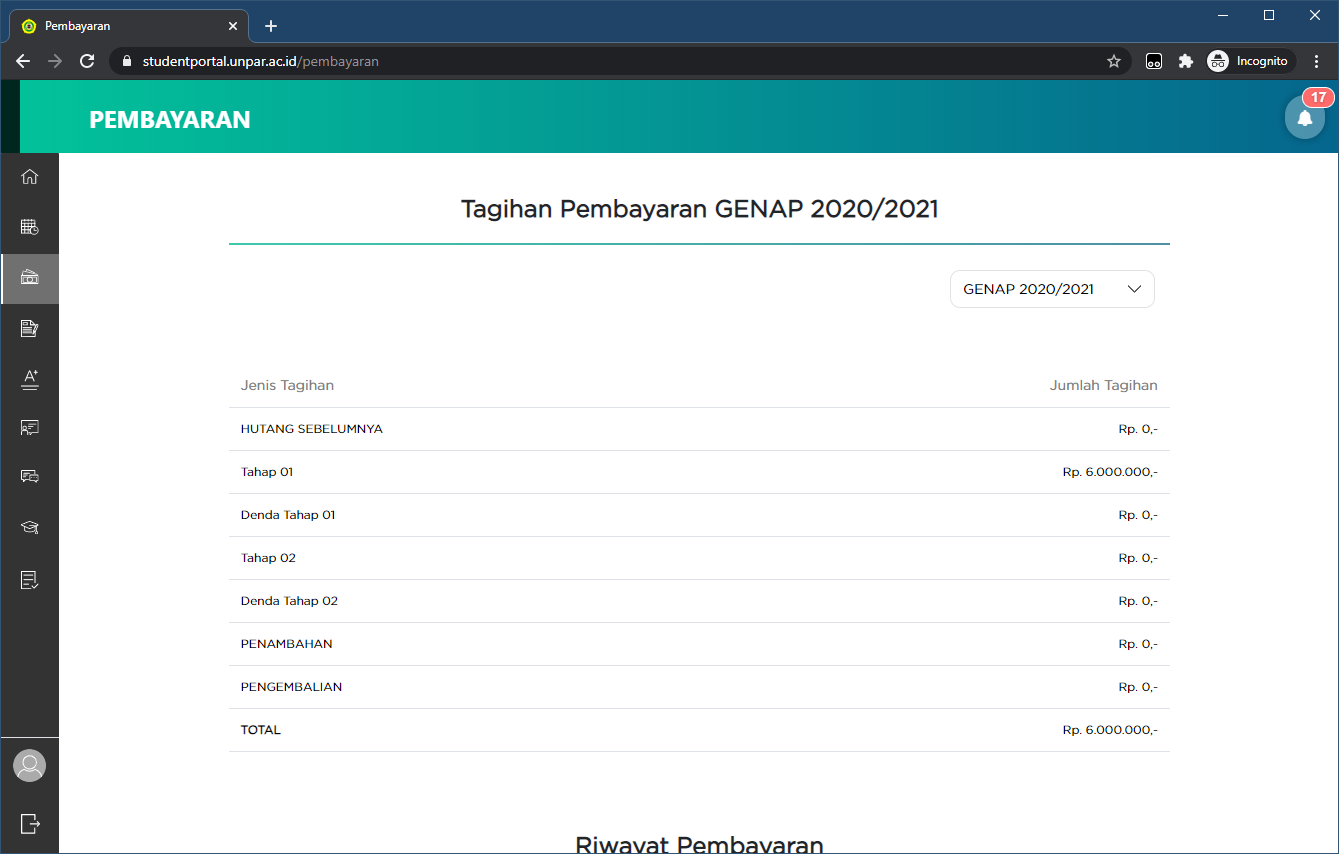
\includegraphics[scale=0.45]{Gambar/pembayaran.png}
		\caption{Halaman Pembayaran}
		\label{fig:3_pembayaran}
	\end{figure}  

\subsection{FRS/PRS}
    Menu FRS/PRS terdiri dari beberapa submenu:
% 		\begin{itemize}
% 			\item FRS/PRS \\
% 			Digunakan sebagai formulir pengisian rencana studi awal (FRS), perubahan rencana studi(PRS) dan menampilkan informasi mata kuliah yang telah diambil saat FRS atau PRS (Gambar \ref{fig:studentportal_frs_prs}).
% 			\begin{figure}[H]
% 				\centering
% 				\includegraphics[scale=0.3]{Gambar/studentportal_frs_prs}
% 				\caption{Tampilan FRS/PRS}
% 				\label{fig:studentportal_frs_prs}
% 			\end{figure}
% 			\item Ubah Jadwal MKU \\
% 			Mahasiswa dapat mengubah jadwal kelas MKU (Gambar \ref{fig:studentportal_ubah_jadwal_mku}).
% 			\begin{figure}[H]
% 				\centering
% 				\includegraphics[scale=0.3]{Gambar/studentportal_ubah_jadwal_mku}
% 				\caption{Tampilan Ubah Jadwal MKU}
% 				\label{fig:studentportal_ubah_jadwal_mku}
% 			\end{figure}
% 		\end{itemize}
	
\subsection{Nilai}
    Menu Nilai terdiri dari beberapa submenu:
    
    \begin{itemize}
        \item Nilai per Semester\\
        Submenu ini menampilkan informasi nilai per semester. Mahasiswa dapat melihat nilai sesuai dengan semester yang dipilih (Gambar \ref{fig:3_nilai_per_semester}). 
        % Semester yang sedang diambil oleh mahasiswa dapat digunakan untuk ditampilkan pada \textit{screensaver}. Pengambilan semester tersebut dilakukan dengan mencari elemen dengan nama "dropdownSemester". 
        
        \begin{figure}[H]
        	\centering
        	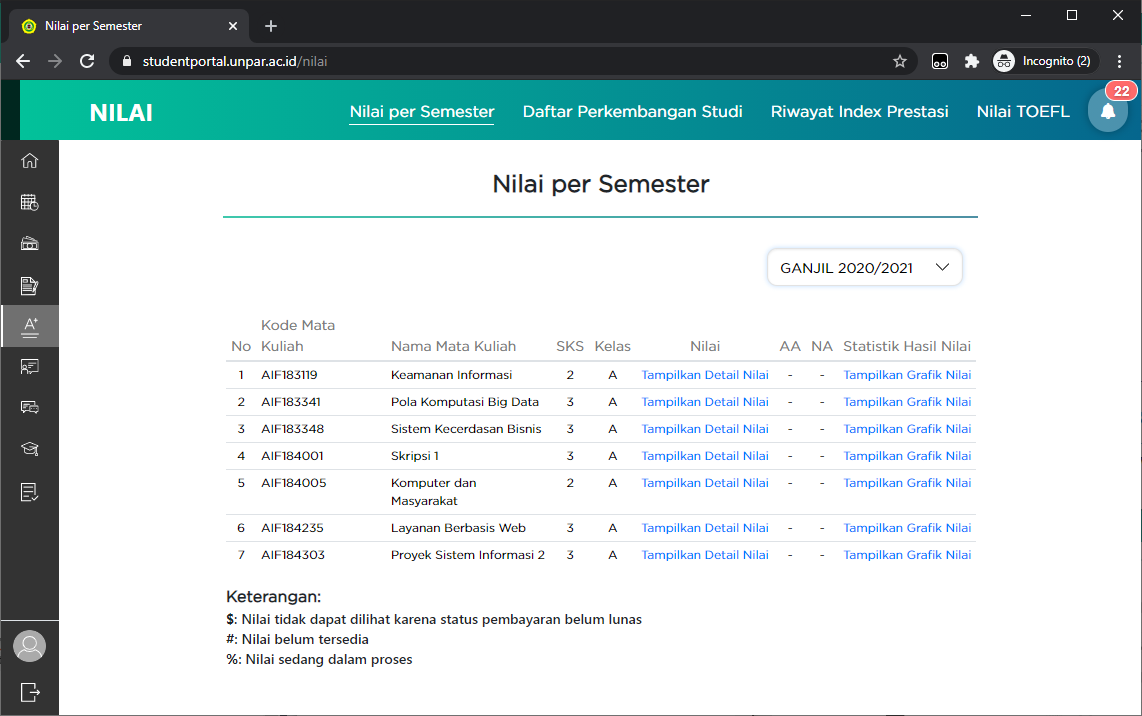
\includegraphics[scale=0.45]{Gambar/nilai_per_semester.png}
        	\caption{Halaman Nilai Per Semester} 
        	\label{fig:3_nilai_per_semester}
        \end{figure}
        
        \item Daftar Perkembangan Studi\\
        Submenu ini menampilkan seluruh riwayat mata kuliah dan nilai yang pernah ditempuh mahasiswa (Gambar \ref{fig:3_dps_1}). Submenu ini juga menampilkan statistik sks, nilai, dan indeks prestasi mahasiswa (Gambar \ref{fig:3_dps_2}).
        \begin{figure}[H]
        	\centering
        	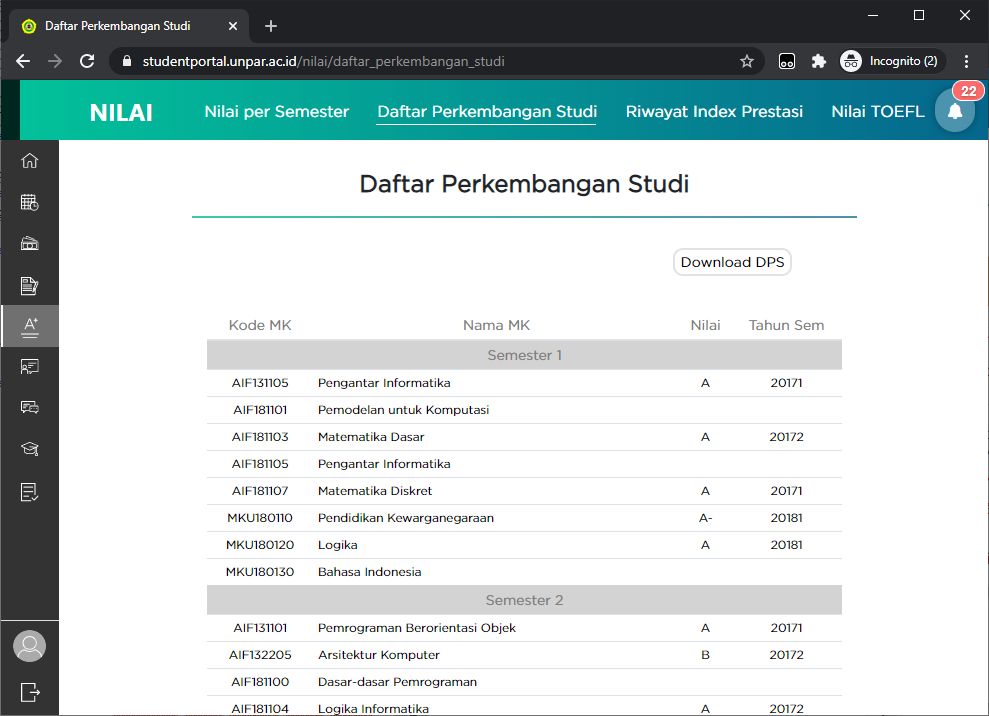
\includegraphics[scale=0.45]{Gambar/nilai_dps_1.png}
        	\caption{Halaman Daftar Perkembangan Studi (1)} 
        	\label{fig:3_dps_1}
        \end{figure}
        
         \begin{figure}[H]
        	\centering
        	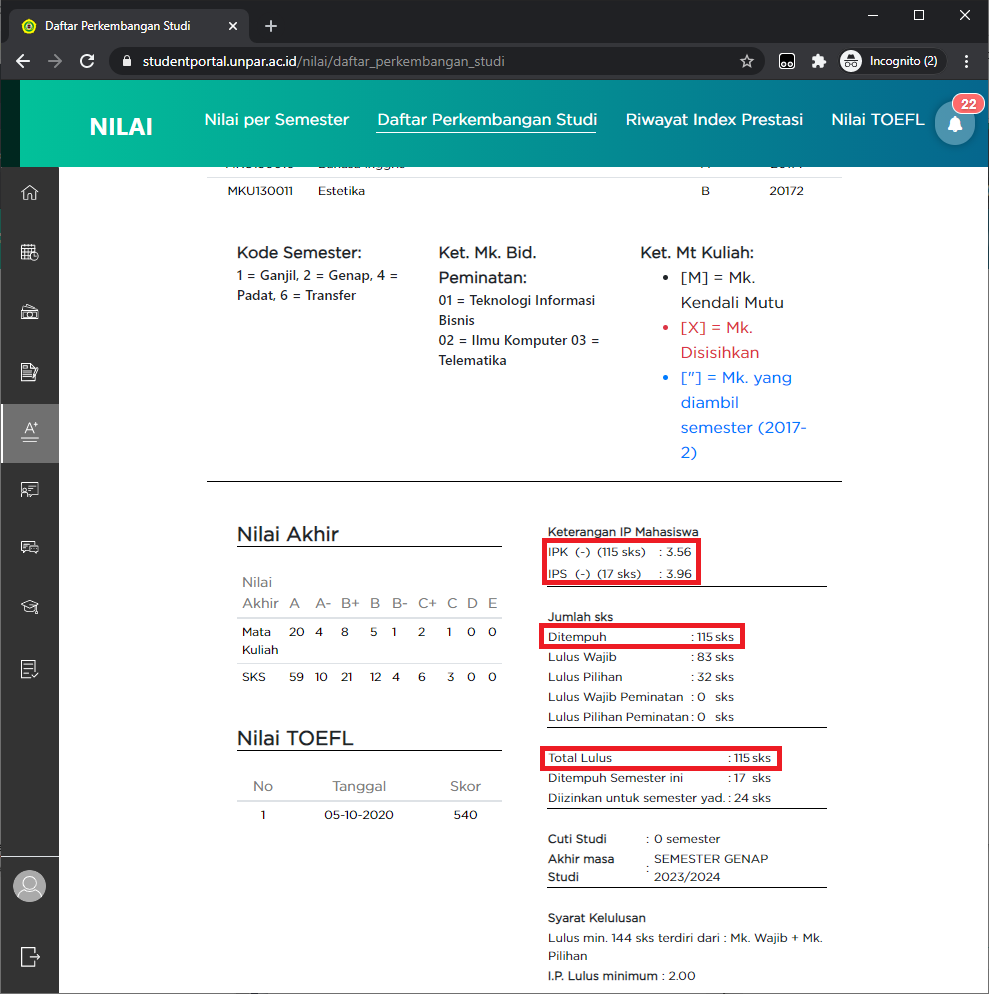
\includegraphics[scale=0.45]{Gambar/nilai_dps_2.png}
        	\caption{Halaman Daftar Perkembangan Studi (2)} 
        	\label{fig:3_dps_2}
        \end{figure}
        Data yang dapat dimanfaatkan dari halaman ini adalah IPK, IPS, jumlah sks yang lulus, dan jumlah sks yang ditempuh. Namun, pada SIAModels sudah terdapat \textit{method} yang melakukan kalkulasi untuk mendapatkan data-data tersebut, sehingga tidak perlu dilakukan pengambilan data menggunakan jsoup. Untuk dapat memanfaatkan \textit{method} tersebut diperlukan seluruh riwayat mata kuliah dan nilai yang pernah ditempuh mahasiswa, sehingga perlu dilakukan pengambilan data menggunakan jsoup.  Implementasi pengambilan data tersebut sudah diimplementasikan sebelumnya pada skripsi Andrianto Sugiarto \cite{ifstupor}. Proses dari pengambilan data tersebut yaitu:
        \begin{itemize}
            \item Mengambil data nilai berdasarkan tahun dan semester dengan mencari elemen "select" yang memiliki id "dropdownSemester", dan memiliki kelas "custom-select mr-3" sehingga kueri css yang dihasilkan adalah "select\#dropdownSemester.custom-select.mr-3".
            \item Dikarenakan perlunya melakukan koneksi berkali-kali sebanyak semester yang telah ditempuh mahasiswa, sehingga dibutuhkan waktu yang tidak sebentar. Karena pada halaman nilai tidak dapat menampilkan seluruh semester seperti Portal Akademik Mahasiswa yang lama, sehingga untuk mengatasi masalah ini dibuat menjadi paralel. Untuk itu dibuat kelas yang mengimplementasikan kelas \textit{interface} \texttt{Runnable}, yaitu kelas \texttt{MultipleRequest}. Kelas inilah yang melakukan koneksi ke setiap semester yang telah ditempuh mahasiswa, dan mengambil data-data tersebut.
        \end{itemize}
        Namun, terdapat beberapa perubahan (Kode \ref{diff_halaman_dps}) yang perlu dilakukan:
        \begin{enumerate}
            \item Menghapus pemanggilan fungsi validateTLSCertificates() dikarenakan sudah \textit{deprecated} \cite{jsoup}.
            \item Indeks yang digunakan untuk melakukan keri css berubah, sehingga untuk mengantisipasi tersebut, indeks yang digunakan menjadi \textit{size} dari kueri css dikurangi 1.
        \end{enumerate}
        
        
        \begin{lstlisting}[language=diff, caption=Perubahan Implementasi Jsoup Halaman Daftar Perkembangan Studi, label=diff_halaman_dps]
@@ -175,7 +175,7 @@ public class Scraper {
        return jadwalList;
}

-   public void requestNilai(String phpsessid, Mahasiswa logged_mhs) throws IOException, InterruptedException {
+       public void requestNilai(String phpsessid) throws IOException, InterruptedException {
            Connection connection = Jsoup.connect(NILAI_URL);
-           connection.cookie("ci_session", phpsessid);
-           connection.timeout(0);
-           connection.validateTLSCertificates(false);
-           connection.method(Connection.Method.POST);
-           Response resp = connection.execute();
-           Document doc = resp.parse();
+           connection.cookie("ci_session", phpsessid);
+           connection.timeout(0);
+           connection.method(Connection.Method.POST);
+           Response resp = connection.execute();
+           Document doc = resp.parse();

-           Elements dropdownSemester = doc.select("#dropdownSemester option");
-           ArrayList<String> listSemester = new ArrayList<String>();
-           for (Element semester : dropdownSemester){
-                   listSemester.add(semester.attr("value"));
-           }
+           Elements dropdownSemester = doc.select("#dropdownSemester option");
+           ArrayList<String> listSemester = new ArrayList<String>();
+           for (Element semester : dropdownSemester){
+               listSemester.add(semester.attr("value"));
+           }

-           Thread[] threadUrl = new Thread[listSemester.size()-1];
-           for(int i = 0; i < listSemester.size()-1; i++){
-               threadUrl[i] = new Thread(new MultipleRequest(i, listSemester, NILAI_URL, phpsessid, logged_mhs));
-               threadUrl[i].start();
-           }
-           for(int i = 0; i < listSemester.size()-1; i++){
-               threadUrl[i].join();
-           }
-           Collections.sort(logged_mhs.getRiwayatNilai(), new Comparator<Nilai>() {
-                   @Override
-                   public int compare(Nilai o1, Nilai o2) {
-                           if (o1.getTahunAjaran() < o2.getTahunAjaran()) {
-                                   return -1;
-                           }
-                           if (o1.getTahunAjaran() > o2.getTahunAjaran()) {
-                                   return + 1;
-                           }
-                           if (o1.getSemester().getOrder() < o2.getSemester().getOrder()) {
-                                   return -1;
-                           }
-                           if (o1.getSemester().getOrder() > o2.getSemester().getOrder()) {
-                                   return +1;
-                           }
-                           return 0;
-                   }
-           });
+           Thread[] threadUrl = new Thread[listSemester.size()-1];
+           for(int i = 0; i < listSemester.size()-1; i++){
+                threadUrl[i] = new Thread(new MultipleRequest(i, listSemester, NILAI_URL, phpsessid, this.mahasiswa));
+                threadUrl[i].start();
+           }
+           for(int i = 0; i < listSemester.size()-1; i++){
+                threadUrl[i].join();
+           }
+           Collections.sort(this.mahasiswa.getRiwayatNilai(), new Comparator<Nilai>() {
+                @Override
+                public int compare(Nilai o1, Nilai o2) {
+                        if (o1.getTahunAjaran() < o2.getTahunAjaran()) {
+                                return -1;
+                        }
+                        if (o1.getTahunAjaran() > o2.getTahunAjaran()) {
+                                return + 1;
+                        }
+                        if (o1.getSemester().getOrder() < o2.getSemester().getOrder()) {
+                                return -1;
+                        }
+                        if (o1.getSemester().getOrder() > o2.getSemester().getOrder()) {
+                                return +1;
+                        }
+                        return 0;
+                }
+           });
        }
        \end{lstlisting}
        
        \item Riwayat Indeks Prestasi\\
       Submenu ini menampilkan seluruh riwayat Indeks Prestasi Semester (IPS) dan Indeks Prestasi Kumulatif (IPK) setiap semester mahasiswa (Gambar \ref{fig:3_rip}).
       
       \begin{figure}[H]
        	\centering
        	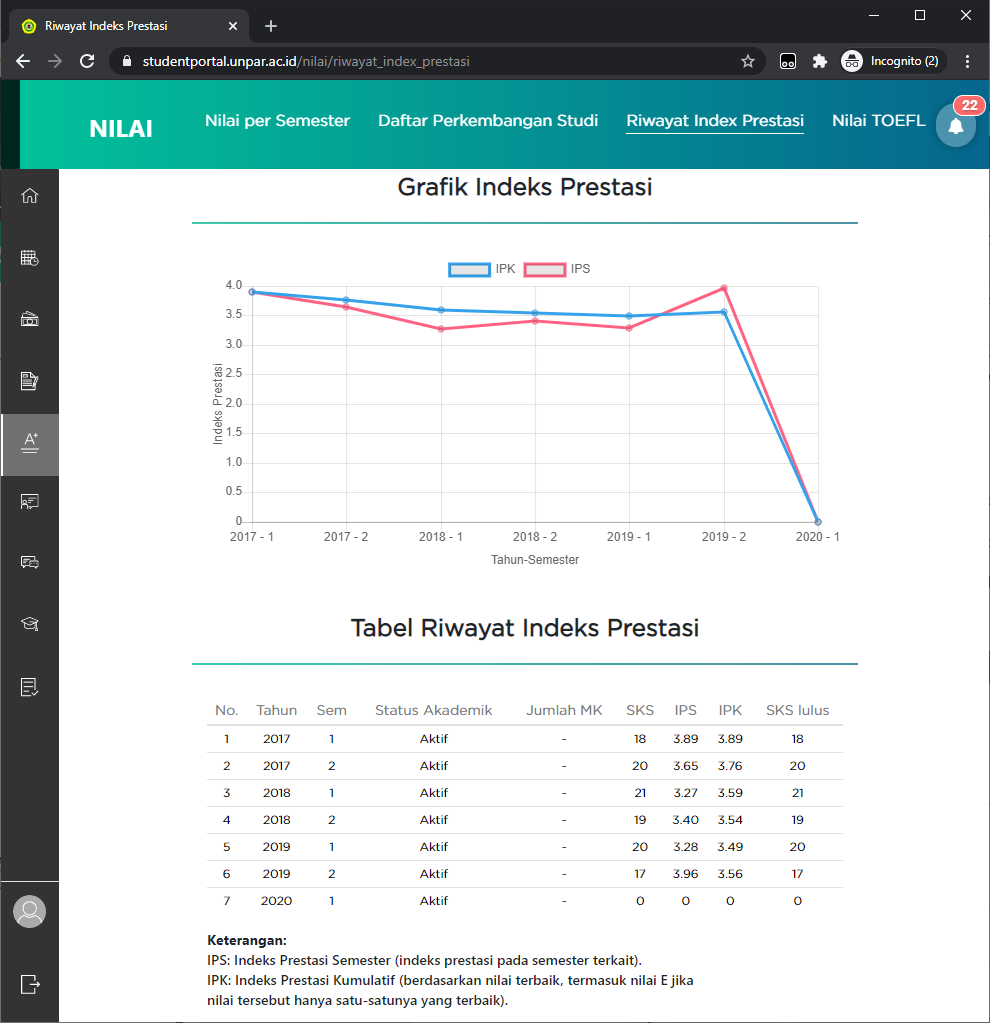
\includegraphics[scale=0.45]{Gambar/nilai_rip.png}
        	\caption{Halaman Riwayat Indeks Prestasi} 
        	\label{fig:3_rip}
        \end{figure}
        
        \item Nilai TOEFL\\
       Submenu ini menampilkan seluruh riwayat skor dan detail skor \textit{Test of English as Foreign Language} (TOEFL) yang pernah ditempuh mahasiswa (Gambar \ref{fig:3_toefl}). Riwayat skor tersebut dapat diambil dengan mencari elemen "table" yang memiliki elemen "tbody" didalamnya, serta memiliki elemen "tr" didalam elemen "tbody".
       Terdapat beberapa perubahan yang terjadi pada halaman TOEFL semenjak skripsi Andrianto Sugiarto \cite{ifstupor}, yang mengakibatkan perlunya perubahan (Kode \ref{diff_toefl}) terhadap implementasi jsoup:

        \begin{enumerate}
            \item Menyimpan atribut mahasiswa pada kelas tersebut agar tidak perlu melakukan \textit{request} \textit{login} berulang kali ketika mengakses menu-menu Portal Akademik Mahasiswa.
            \item Menghapus pemanggilan fungsi validateTLSCertificates() dikarenakan sudah \textit{deprecated} \cite{jsoup}.
            \item Perubahan format tanggal TOEFL pada Portal Akademik Mahasiswa menjadi dd-mm-yyyy.
        \end{enumerate}
       
       \begin{figure}[H]
        	\centering
        	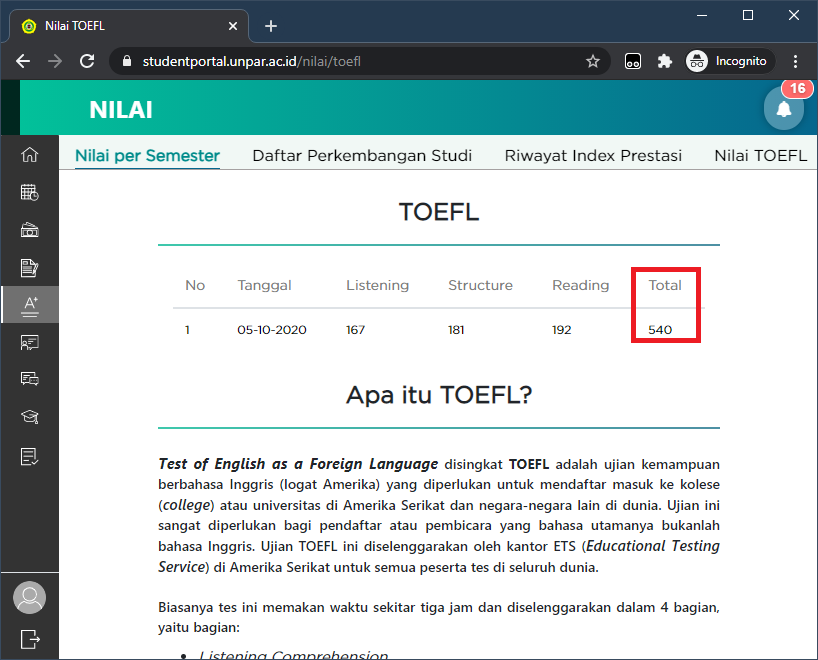
\includegraphics[scale=0.45]{Gambar/nilai_toefl.png}
        	\caption{Halaman Nilai TOEFL} 
        	\label{fig:3_toefl}
        \end{figure}
        

        \begin{lstlisting}[language=diff, caption=Perubahan Implementasi Jsoup TOEFL, label=diff_toefl]
@@ -218,68 +218,29 @@ public class Scraper {
        });
}

-       public void requestNilaiTOEFL(String phpsessid, Mahasiswa mahasiswa) throws IOException {
-           SortedMap<LocalDate, Integer> nilaiTerakhirTOEFL = new TreeMap<>();
-           Connection connection = Jsoup.connect(TOEFL_URL);
-           connection.cookie("ci_session", phpsessid);
-           connection.timeout(0);
-           connection.validateTLSCertificates(false);
-           connection.method(Connection.Method.POST);
-           Response resp = connection.execute();
-           Document doc = resp.parse();
-           Elements nilaiTOEFL = doc.select("table").select("tbody").select("tr");
-           if (!nilaiTOEFL.isEmpty()) {
-               for (int i = 0; i < nilaiTOEFL.size(); i++) {
-                   Element nilai = nilaiTOEFL.get(i).select("td").get(5);
-                   Element tgl_toefl = nilaiTOEFL.get(i).select("td").get(1);
-                   String[] tanggal = tgl_toefl.text().split(" ");
-                   switch (tanggal[1].toLowerCase()) {
-                   case "januari":
-                       tanggal[1] = "1";
-                       break;
-                   case "februari":
-                       tanggal[1] = "2";
-                       break;
-                   case "maret":
-                       tanggal[1] = "3";
-                       break;
-                   case "april":
-                       tanggal[1] = "4";
-                       break;
-                   case "mei":
-                       tanggal[1] = "5";
-                       break;
-                   case "juni":
-                       tanggal[1] = "6";
-                       break;
-                   case "juli":
-                       tanggal[1] = "7";
-                       break;
-                   case "agustus":
-                       tanggal[1] = "8";
-                       break;
-                   case "september":
-                       tanggal[1] = "9";
-                       break;
-                   case "oktober":
-                       tanggal[1] = "10";
-                       break;
-                   case "november":
-                       tanggal[1] = "11";
-                       break;
-                   case "desember":
-                       tanggal[1] = "12";
-                       break;
-                   }
+       public void requestNilaiTOEFL(String phpsessid) throws IOException {
+           SortedMap<LocalDate, Integer> nilaiTerakhirTOEFL = new TreeMap<>();
+           Connection connection = Jsoup.connect(TOEFL_URL);
+           connection.cookie("ci_session", phpsessid);
+           connection.timeout(0);
+           connection.method(Connection.Method.POST);
+           Response resp = connection.execute();
+           Document doc = resp.parse();
+           Elements nilaiTOEFL = doc.select("table").select("tbody").select("tr");
+           if (!nilaiTOEFL.isEmpty()) {
+               for (int i = 0; i < nilaiTOEFL.size(); i++) {
+                   Element nilai = nilaiTOEFL.get(i).select("td").get(5);
+                   Element tgl_toefl = nilaiTOEFL.get(i).select("td").get(1);
+                   String[] tanggal = tgl_toefl.text().split("-");

-                   LocalDate localDate = LocalDate.of(Integer.parseInt(tanggal[2]), Integer.parseInt(tanggal[1]),
-                                       Integer.parseInt(tanggal[0]));
+                   LocalDate localDate = LocalDate.of(Integer.parseInt(tanggal[2]), Integer.parseInt(tanggal[1]),
+                                       Integer.parseInt(tanggal[0]));

-                   nilaiTerakhirTOEFL.put(localDate, Integer.parseInt(nilai.text()));
-               }
-           }
-           mahasiswa.setNilaiTOEFL(nilaiTerakhirTOEFL);
-       }
+                   nilaiTerakhirTOEFL.put(localDate, Integer.parseInt(nilai.text()));
+               }
+           }
+           this.mahasiswa.setNilaiTOEFL(nilaiTerakhirTOEFL);
+       }
        \end{lstlisting}

    \end{itemize}
    
\subsection{Angket}
    Menu Angket merupakan halaman dimana mahasiswa diminta untuk mengisi angket dari para dosen yang mengajarnya di semester yang sedang ditempuh mahasiswa tersebut (Gambar \ref{fig:3_angket}).
        \begin{figure}[H]
        	\centering
        	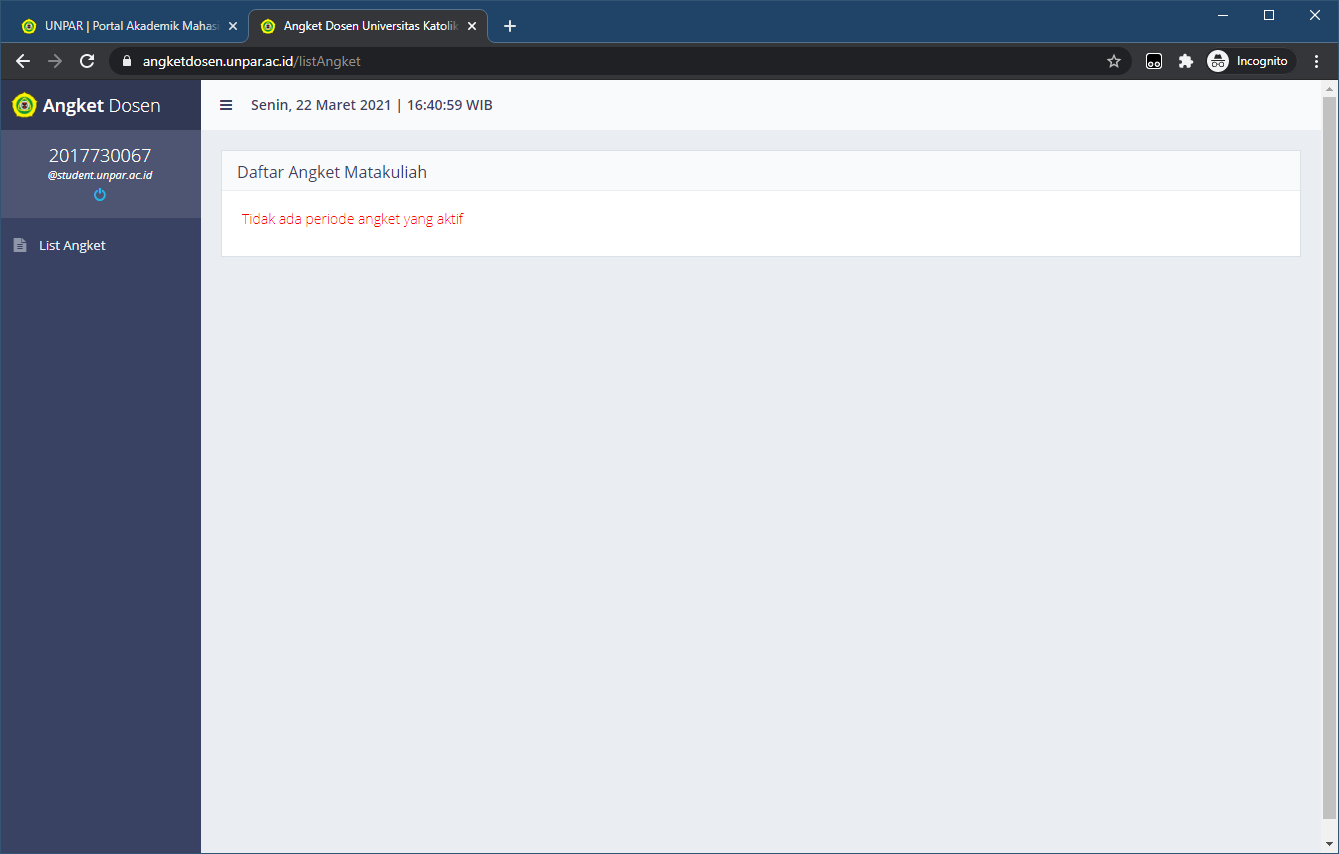
\includegraphics[scale=0.45]{Gambar/angket.png}
        	\caption{Halaman Angket} 
        	\label{fig:3_angket}
        \end{figure}
        
\subsection{Saran \& Komentar}
    Menu Saran \& Komentar akan membuka halaman \url{https://suaramahasiswa.unpar.ac.id/} (Gambar \ref{fig:3_saran_komentar}).
    \begin{figure}[H]
    	\centering
    	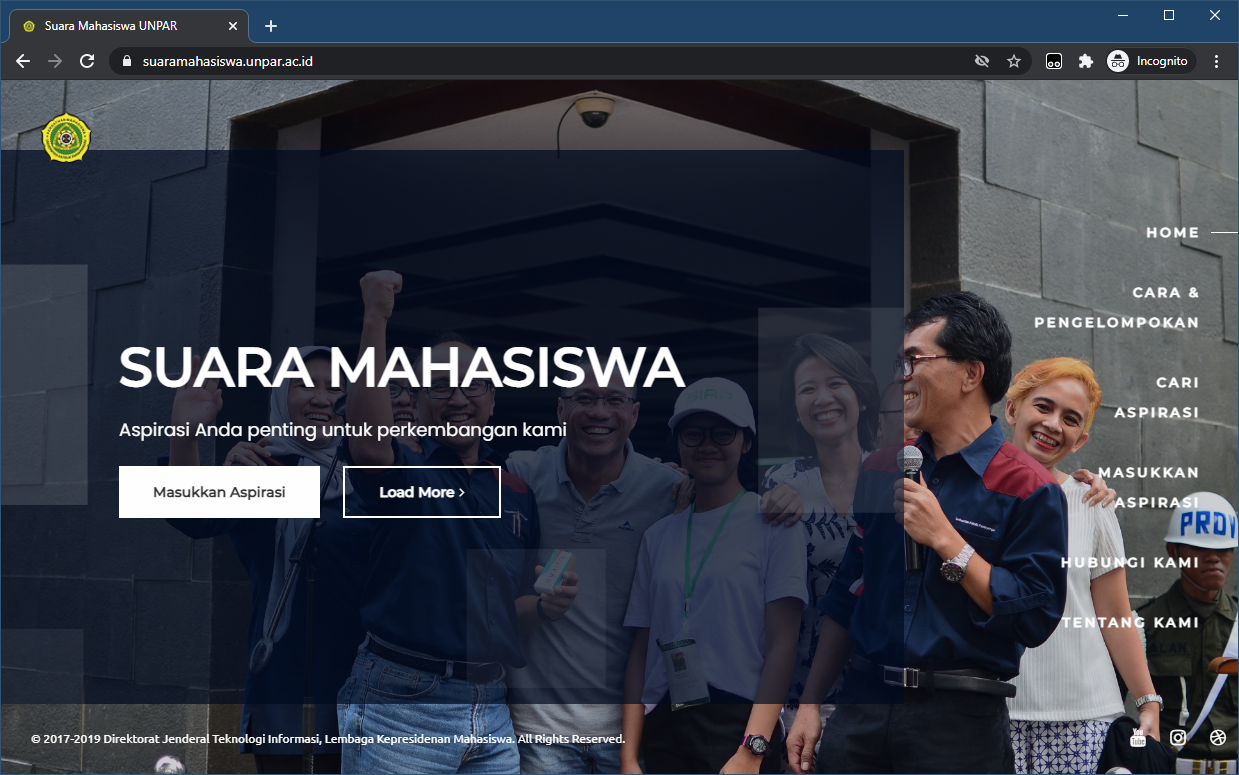
\includegraphics[scale=0.45]{Gambar/sarankomentar.png}
    	\caption{Halaman Saran \& Komentar} 
    	\label{fig:3_saran_komentar}
    \end{figure}
        
\subsection{Kelulusan}
    Menu Kelulusan sedang dalam tahap pembangunan (Gambar \ref{fig:3_kelulusan}).
    \begin{figure}[H]
    	\centering
    	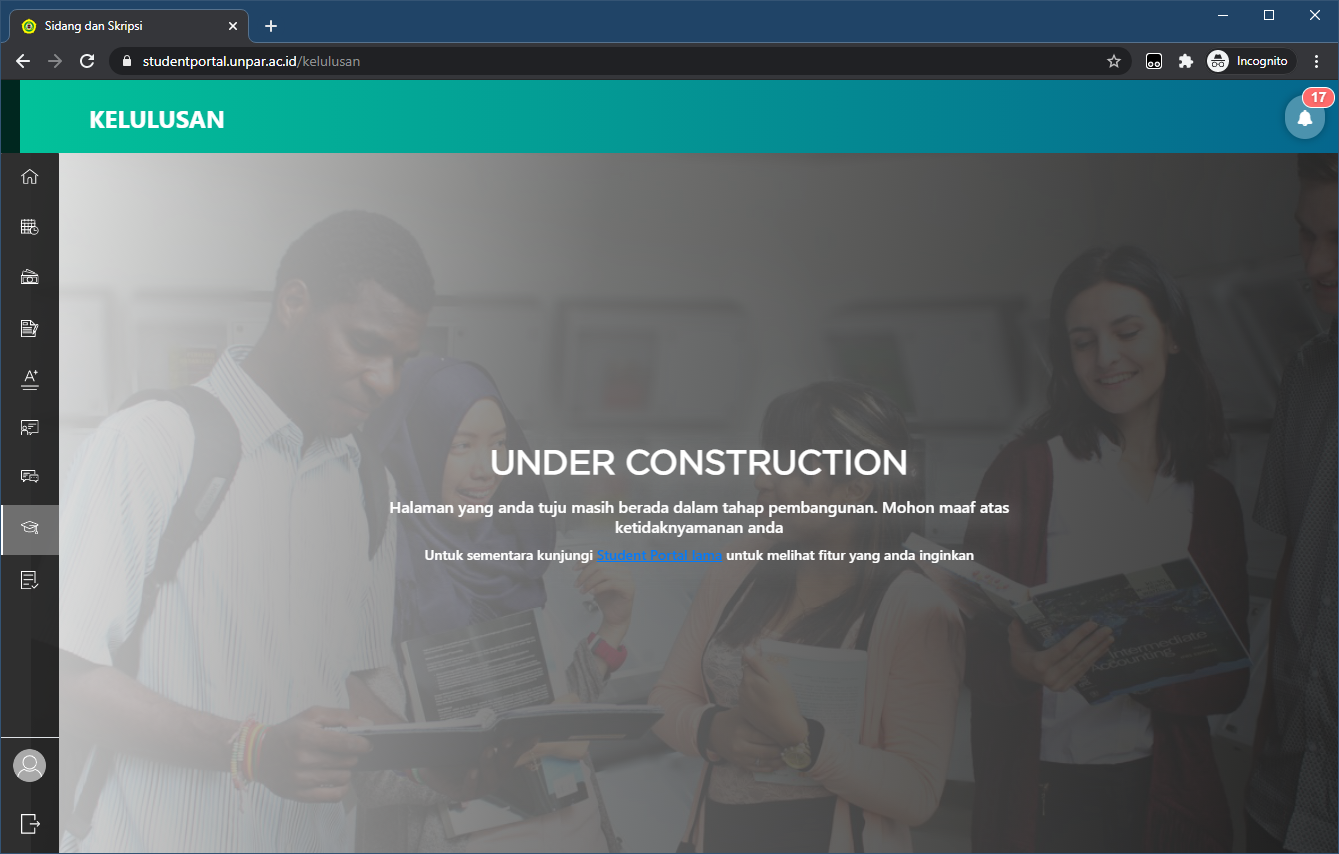
\includegraphics[scale=0.45]{Gambar/kelulusan.png}
    	\caption{Halaman Kelulusan} 
    	\label{fig:3_kelulusan}
    \end{figure}

\subsection{Pengajuan}
    Menu Pengajuan merupakan halaman dimana mahasiswa dapat mengajukan topik skripsi atau tugas akhir (Gambar \ref{fig:3_pengajuan}).
    \begin{figure}[H]
    	\centering
    	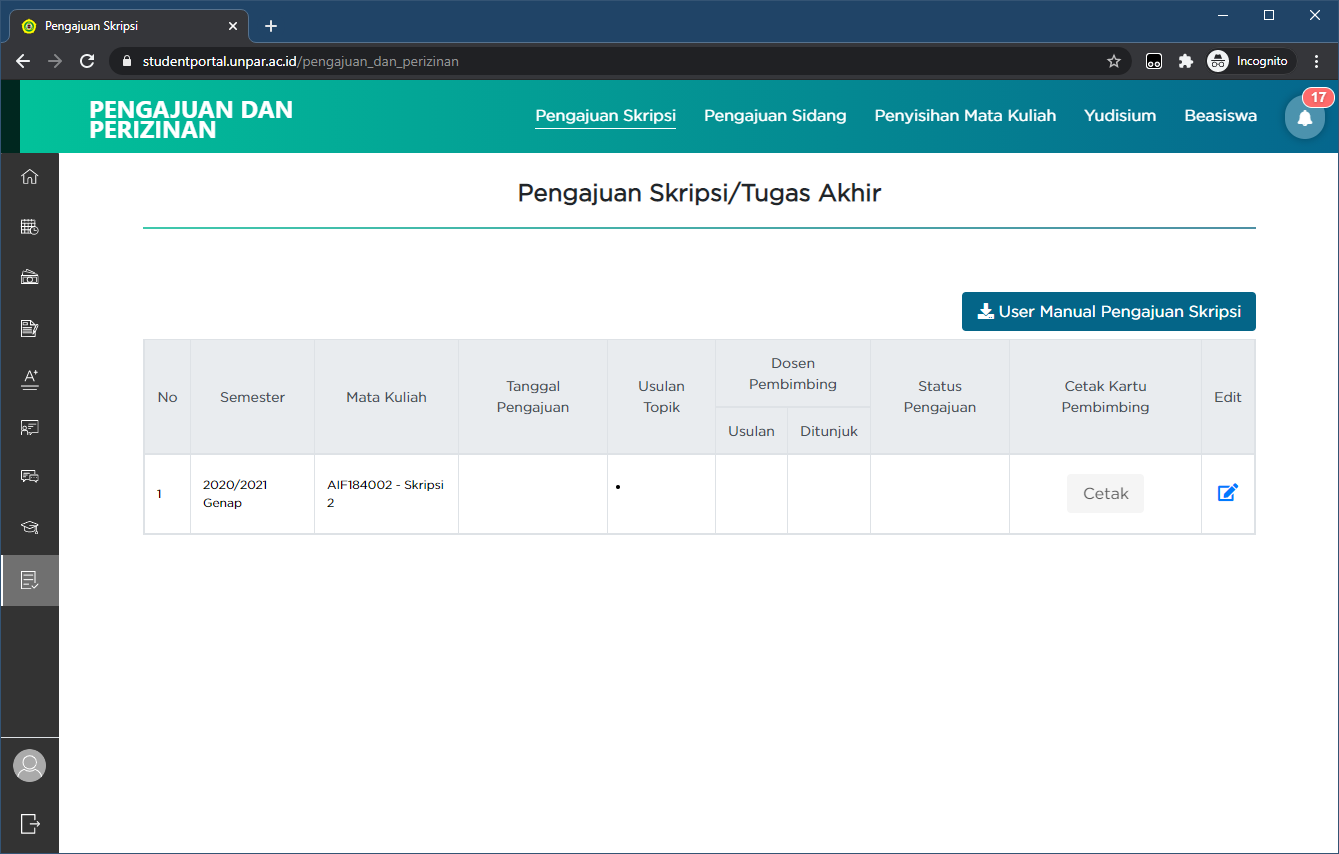
\includegraphics[scale=0.45]{Gambar/pengajuan.png}
    	\caption{Halaman Pengajuan} 
    	\label{fig:3_pengajuan}
    \end{figure}